\documentclass[12pt]{article}
\usepackage{amsthm,amssymb,amsfonts,amsmath,amstext,systeme}
\usepackage{graphicx,float}
\usepackage{tabularx}

\marginparwidth 0pt
\oddsidemargin -1.2 truecm
\evensidemargin  0pt 
\marginparsep 0pt
\topmargin -2.2truecm
\linespread{1}
\textheight 25.8 truecm
\textwidth 18.5 truecm
\newenvironment{remark}{\noindent{\bf Remark }}{\vspace{0mm}}
\newenvironment{remarks}{\noindent{\bf Remarks }}{\vspace{0mm}}
\newenvironment{question}{\noindent{\bf Question }}{\vspace{0mm}}
\newenvironment{questions}{\noindent{\bf Questions }}{\vspace{0mm}}
\newenvironment{note}{\noindent{\bf Note }}{\vspace{0mm}}
\newenvironment{summary}{\noindent{\bf Summary }}{\vspace{0mm}}
\newenvironment{back}{\noindent{\bf Background}}{\vspace{0mm}}
\newenvironment{conclude}{\noindent{\bf Conclusion}}{\vspace{0mm}}
\newenvironment{concludes}{\noindent{\bf Conclusions}}{\vspace{0mm}}
\newenvironment{dill}{\noindent{\bf Description of Dill's model}}{\vspace{0mm}}
\newenvironment{maths}{\noindent{\bf Mathematics needed}}{\vspace{0mm}}
\newenvironment{inst}{\noindent{\bf Instructions}}{\vspace{0mm}}
\newenvironment{notes}{\noindent{\bf Notes }}{\vspace{0mm}}
\newenvironment{theorem}{\noindent{\bf Theorem }}{\vspace{0mm}}
\newenvironment{example}{\noindent{\bf Example }}{\vspace{0mm}}
\newenvironment{examples}{\noindent{\bf Examples }}{\vspace{0mm}}
\newenvironment{topics}{\noindent{\bf Topics}}{\vspace{0mm}}
\newenvironment{outcomes}{\noindent{\bf Expected Learning Outcomes}}{\vspace{0mm}}
\newenvironment{lemma}{\noindent{\bf Lemma }}{\vspace{0mm}}
\newenvironment{solution}{\noindent{\it Solution}}{\vspace{2mm}}
\newcommand{\ds}{\displaystyle}
\newcommand{\un}{\underline}
\newcommand{\bs}{\boldsymbol}

\begin{document}

\baselineskip 18 pt
\begin{center}
	{\large \bf HKDSE MATH CORE 2014 Past Paper I}\\
	\vspace{2 mm}

\end{center}
\vspace{0.05cm}

\begin{enumerate}
	\item \textbf{HKDSE MATH CORE 2014 Past Paper I Q1}\\
	Simplify $\dfrac{(xy^{-2})^3}{y^4}$ and express your answer with positive indices. \\(3 marks)	
	
	\item \textbf{HKDSE MATH CORE 2014 Past Paper I Q2}\\
	Factorize
	\begin{enumerate}
		\item [(a)] $a^2 - 2a - 3$,
		\item [(b)] $ab^2 + b^2 + a^2 - 2a - 3 + 6m - 15n$.
	\end{enumerate}
	(3 marks)

	\item \textbf{HKDSE MATH CORE 2014 Past Paper I Q3}
	\begin{enumerate}
		\item[(a)] Round up 123.45 to 1 significant figure.
		\item[(b)] Round off 123.45 to the nearest integer.
		\item[(c)] Round down 123.45 to 1 decimal place.	
	\end{enumerate}
	(3 marks)

	\item \textbf{HKDSE MATH CORE 2014 Past Paper I Q4}\\
	The table below shows the distribution of the numbers of calculators owned by some students.
	$$\begin{array}{|c|c|c|c|c|}
		\hline
		\text{Number of calculators} & 0 & 1 & 2 & 3 \\
		\hline
		\text{Number of students} & 7 & 14 & 15 & 4 \\
		\hline
	\end{array}$$
	Find the median, the mode and the standard deviation of the above distribution. \\(3 marks)

	\item \textbf{HKDSE MATH CORE 2014 Past Paper I Q5}\\
	Consider the formula $2(3m +n) = m + 7$.
	\begin{enumerate}
		\item[(a)] Make $n$ the subject of the above formula.
		\item[(b)] If the value of $m$ is increased by 2, write down the change in the value of $n$.	
	\end{enumerate}
	(4 marks)

	\item \textbf{HKDSE MATH CORE 2014 Past Paper I Q6}\\
	The marked price of a toy is \$255. The toy is now sold at a discount of 40\% on its marked price.
	\begin{enumerate}
		\item[(a)] Find the selling price of the toy.
		\item[(b)] If the percentage profit is 2\%, find the cost of the toy.		
	\end{enumerate}
	(4 marks)

	\item \textbf{HKDSE MATH CORE 2014 Past Paper I Q7}\\
	Let $f(x) = 4x^3 - 5x^2 - 18x + c$, where $c$ is a constant. When  $f(x)$ is divided by $x - 2$, the remainder is $-33$.
	\begin{enumerate}
		\item[(a)] Is $x + 1$ a factor of $f(x)$? Explain your answer.
		\item[(b)] Someone claims that all the roots of the equation  $f(x) = 0$ are rational numbers. Do you agree? Explain your answer.
	\end{enumerate}
	(5 marks)
	
	\item \textbf{HKDSE MATH CORE 2014 Past Paper I Q8}\\
	The coordinates of the points $P$ and $Q$ are $(-3, 5)$ and $(2, -7)$ respectively. $P$ is rotated anticlockwise about the origin $O$ through $270^\circ$ to $P'$. $Q$ is translated leftwards by 21 units to $Q'$.
	\begin{enumerate}
		\item[(a)] Write down the coordinates of $P'$ and $Q'$.
		\item[(b)] Prove that PQ is perpendicular to $P'Q'$.
	\end{enumerate}
	(5 marks)

	\item \textbf{HKDSE MATH CORE 2014 Past Paper I Q9}\\
	In Figure 1, $D$ is a point lying on $AC$ such that $\angle BAC = \angle CBD$.		
	\begin{figure}[H]
		\centering
		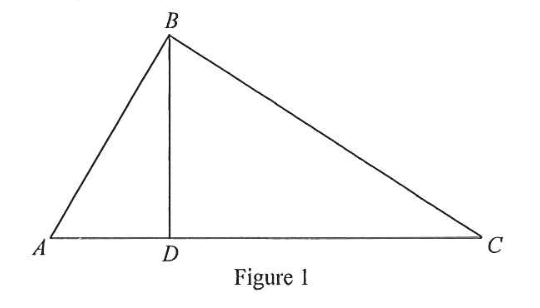
\includegraphics[width = .3\linewidth]{2014Figure1.1}
	\end{figure}
	\begin{enumerate}
		\item[(a)] Prove that $\triangle ABC \sim \triangle BDC$.
		\item[(b)] Suppose that $AC = 25$ cm, $BC = 20$ cm and $BD = 12$ cm. Is $\triangle BCD$ a right-angled triangle? Explain your answer.
	\end{enumerate}
	(5 marks)

	\item \textbf{HKDSE MATH CORE 2014 Past Paper I Q10}\\
	Town $X$ and town $Y$ are 80 km apart. Figure 2 shows the graphs for car $A$ and car $B$ travelling on the same straight road between town $X$ and town $Y$ during the period 7:30 to 9:30 in a morning. Car $A$ travels at a constant speed during the period. Car $B$ comes to rest at 8:15 in the morning.
	\begin{figure}[H]
		\centering
		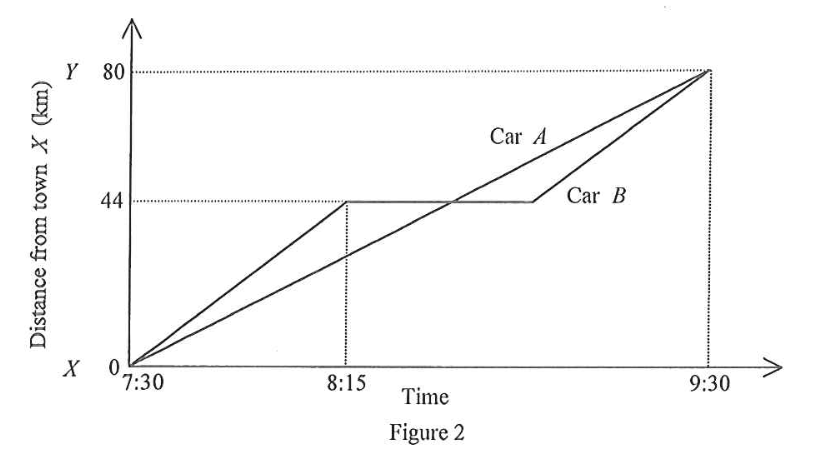
\includegraphics[width = .3\linewidth]{2014Figure1.2}
	\end{figure}
	\begin{enumerate}
		\item[(a)] Find the distance of car $A$ from town $X$ at 8:15 in the morning. \\(2 marks)
		\item[(b)] At what time after 7:30 in the morning do car $A$ and car $B$ first meet? \\(2 marks)
		\item[(c)] The driver of car $B$ claims that the average speed of car $B$ is higher than that of car $A$ during the period 8:15 to 9:30 in the morning. Do you agree? Explain your answer. \\(2 marks)
	\end{enumerate}

	\item \textbf{HKDSE MATH CORE 2014 Past Paper I Q11}\\
	There are 33 paintings in an art gallery. The box-and-whisker diagram below shows the distribution of the prices (in thousand dollars) of the paintings in the art gallery. It is given that the mean of this distribution is 53 thousand dollars.
	\begin{figure}[H]
		\centering
		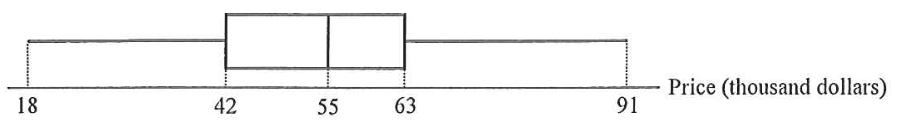
\includegraphics[width = .3\linewidth]{2014Figure1.00}
	\end{figure}
	\begin{enumerate}
		\item[(a)] Find the range and the inter-quartile range of the above distribution. \\(3 marks)
		\item[(b)] Four paintings of respective prices (in thousand dollars) 32, 34, 58 and 59 are now donated to a museum. Find the mean and the median of the prices of the remaining paintings in the art gallery. \\(3 marks)
	\end{enumerate}

	\item \textbf{HKDSE MATH CORE 2014 Past Paper I Q12}\\
	The circle $C$ passes through the point $A(6, 11)$ and the centre of $C$ is the point $G(0, 3)$.
	\begin{enumerate}
		\item[(a)] Find the equation of $C$. \\(2 marks)
		\item[(b)] $P$ is a moving point in the rectangular coordinate plane such that $AP = GP$. Denote the locus of $P$ by $\Gamma$.
		\begin{enumerate}
			\item[(i)] Find the equation of $\Gamma$.
			\item[(ii)] Describe the geometric relationship between $\Gamma$ and the line segment $AG$.
			\item[(iii)] If $\Gamma$ cuts $C$ at $Q$ and $R$, find the perimeter of the quadrilateral $AQGR$.	
		\end{enumerate}
		(5 marks)
	\end{enumerate}

	\item \textbf{HKDSE MATH CORE 2014 Past Paper I Q13}\\
	It is given that $f(x)$ is the sum of two parts, one part varies as $x^2$ and the other part is a constant. Suppose that $f(2) = 59$ and $f(7) = -121$.
	\begin{enumerate}
		\item[(a)] Find $f(6)$. \\(4 marks)
		\item[(b)] $A(6, a)$ and $B(-6, b)$ are points lying on the graph of $y = f(x)$. Find the area of $\triangle ABC$, where $C$ is a point lying on the $x$-axis. \\(4 marks)
	\end{enumerate}

	\item \textbf{HKDSE MATH CORE 2014 Past Paper I Q14}\\
	Figure 3 shows a vessel in the form of a frustum which is made by cutting off the lower part of an inverted right circular cone of base radius 72 cm and height 96 cm. The height of the vessel is 60 cm. The vessel is placed on a horizontal table. Some water is now poured into the vessel. John finds that the depth of the water in the vessel is 28 cm.
	\begin{figure}[H]
		\centering
		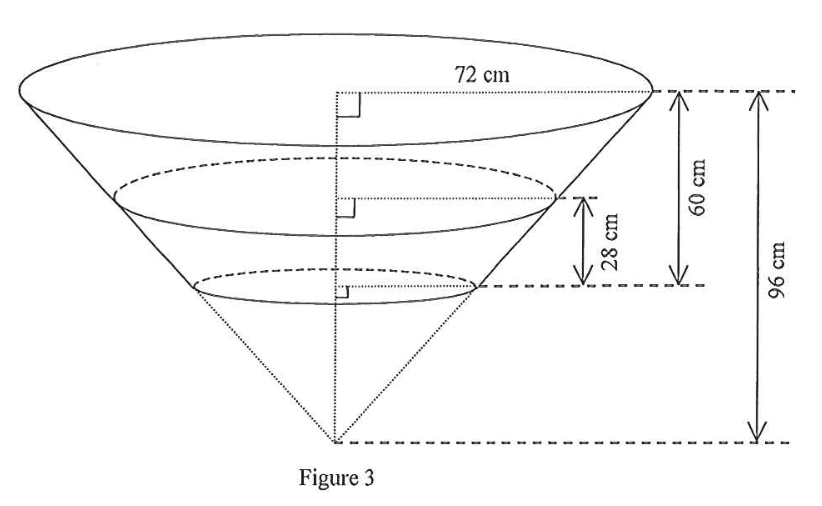
\includegraphics[width = .3\linewidth]{2014Figure1.3}
	\end{figure}
	\begin{enumerate}
		\item[(a)] Find the area of the wet curved surface of the vessel in terms of $\pi$. \\(4 marks)
		\item[(b)] John claims that the volume of water in the vessel is greater than 0.1 m$^3$. Do you agree? Explain your answer. \\(4 marks)
	\end{enumerate}

	\item \textbf{HKDSE MATH CORE 2014 Past Paper I Q15}\\
	The graph in Figure 4 shows the linear relation between $\log_4x$ and $\log_8y$. The slope and the intercept on the horizontal axis are $\dfrac{-1}{3}$ and 3 respectively. Express the relation between $x$ and $y$ in the form $y = Ax^k$, where $A$ and $k$ are constants. \\(3 marks)
	\begin{figure}[H]
		\centering
		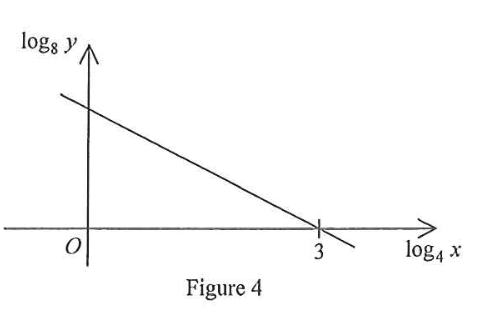
\includegraphics[width = .3\linewidth]{2014Figure1.4}
	\end{figure}


	\item \textbf{HKDSE MATH CORE 2014 Past Paper I Q16}\\
	In figure 5, the 1st pattern consists of 3 dots. For any positive integer $n$, the $(n + 1)$th pattern is formed by adding 2 dots to the nth pattern. Find the least value of m such that the total number of dots in the first $m$ patterns exceeds 6 888. \\(4 marks)
	\begin{figure}[H]
		\centering
		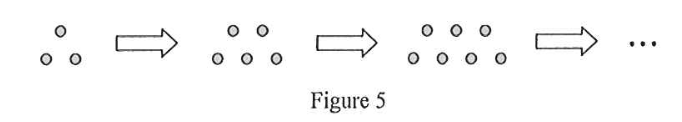
\includegraphics[width = .3\linewidth]{2014Figure1.5}
	\end{figure}

	\item \textbf{HKDSE MATH CORE 2014 Past Paper I Q17}\\
	Figure 6(a) shows a solid pyramid $VABCD$ with a rectangular base, where $AB = 18$ cm, $BC = 10$ cm, $VB = VC = 30$ cm and $\angle VAB = \angle VDC = 110^\circ$.
	\begin{figure}[H]
		\centering
		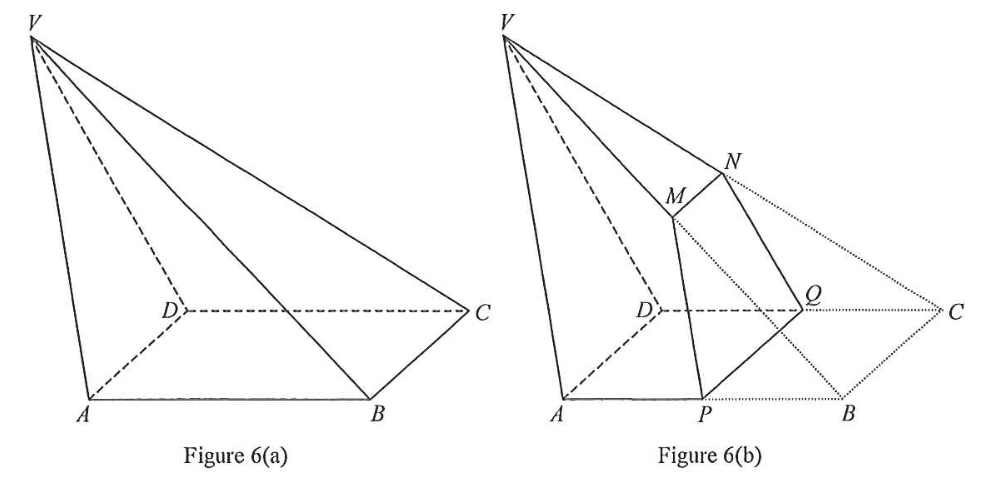
\includegraphics[width = .3\linewidth]{2014Figure1.6}
	\end{figure}
	\begin{enumerate}
		\item[(a)] Find $\angle VBA$. \\(2 marks)
		\item[(b)] $P$, $Q$, $M$ and $N$ are the mid-points of $AB$, $CD$, $VB$ and $VC$ respectively. A geometric model is made by cutting off $PBCQNM$ from $VABCD$ as shown in Figure 6(b). A craftsman claims that the area of the trapezium $PQNM$ is less than 70 cm$^2$. Do you agree? Explain your answer. \\(5 marks)
	\end{enumerate}

	\item \textbf{HKDSE MATH CORE 2014 Past Paper I Q18}
	\begin{enumerate}
		\item[(a)] In Figure 7, the equation of the straight line $L_1$ is $6x + 7y = 900$ and the $x$-intercept of the straight line $L_2$ is 180. $L_1$ and $L_2$ intersect at the point $(45, 90)$. The shaded region (including the boundary) represents the solution of a system of inequalities. Find the system of inequalities.											
		\begin{figure}[H]
			\centering
			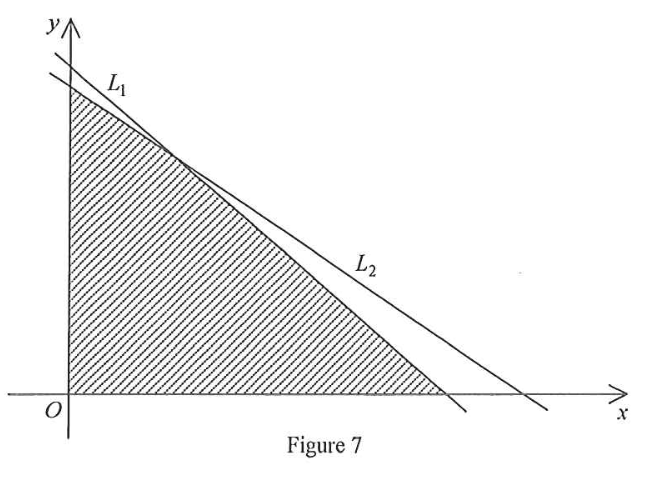
\includegraphics[width = .3\linewidth]{2014Figure1.7}
		\end{figure}
		\item[(b)] A factory produces two types of wardrobes, $X$ and $Y$. Each wardrobe $X$ requires 6 man-hours for assembly and 2-man hours for packing while each wardrobe $Y$ requires 7 man-hours for assembly and 3 man-hours for packing. In a certain month, the factory has 900 man-hours available for assembly and 360 man-hours available for packing. The profits for producing a wardrobe $X$ and a wardrobe $Y$ are \$440 and \$665 respectively. A worker claims that the total profit can exceed \$80 000 that month. Do you agree? Explain your answer. \\(4 marks)
	\end{enumerate}

	\item \textbf{HKDSE MATH CORE 2014 Past Paper I Q19}\\
	Ada and Billy play a game consisting of two rounds. In the first round, Ada and Billy take turns to throw a fair die. The player who first gets a number '3' wins the first round. Ada and Billy play the first round until one of them wins. Ada throws the die first.
	\begin{enumerate}
		\item[(a)] Find the probability that Ada wins the first round of the game. \\(3 marks)
		\item[(b)] In the second round of the game, balls are dropped one by one into a device containing eight tubes arranged side by side (see Figure 8). When a ball is dropped into the device, it falls randomly into one of the tubes. Each tube can hold at most three balls.
		\begin{figure}[H]
			\centering
			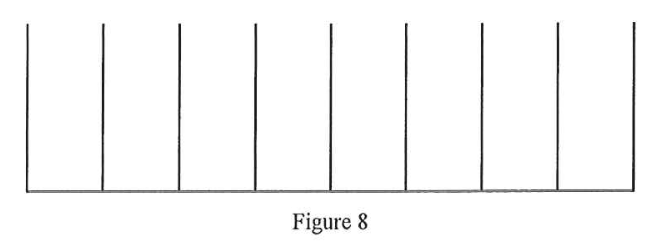
\includegraphics[width = .3\linewidth]{2014Figure1.8}
		\end{figure}
		The player of this round adopts one of the following two options.
		\begin{enumerate}
			\item[Option 1:] Two balls are dropped one by one into the device. If the two balls fall into the same tube, then the player gets 10 tokens. If the two balls fall into two adjacent tubes, then the player gets 5 tokens. Otherwise, the player gets no tokens.
			\item[Option 2:] Three balls are dropped one by one into the device. If the three balls fall into the same tube, then the player gets 50 tokens. If the three balls fall into three adjacent tubes, then the player gets 10 tokens. If the three balls fall into two adjacent tubes, then the player gets 5 tokens. Otherwise, the player gets no tokens.
		\end{enumerate}
		\begin{enumerate}
			\item[(i)] If the player of the second round adopts Option 1, find the expected number of tokens got.
			\item[(ii)] Which option should the player of the second round adopt in order to maximise the expected number of tokens got? Explain your answer.
			\item[(iii)] Only the winner of the first round plays the second round. It is given that the player of the second round adopts the option which can maximise the expected number of tokens got. Billy claims that the probability of Ada getting no tokens in the game exceeds 0.9. Is the claim correct? Explain your answer.
		\end{enumerate}
		(10 marks)
	\end{enumerate}
\end{enumerate}


\end{document}